
\section*{TEE identification}

Remote attestation is a key feature of SGX, and other similar TEE architectures, as it allows a remote verifier to check that the attested enclave was correctly constructed before provisioning secrets to it. 

\begin{figure}[t]
 \centering
  %\includegraphics[trim={0 13.4cm 11cm 0},clip,width=\linewidth]{relayAttack.pdf}
  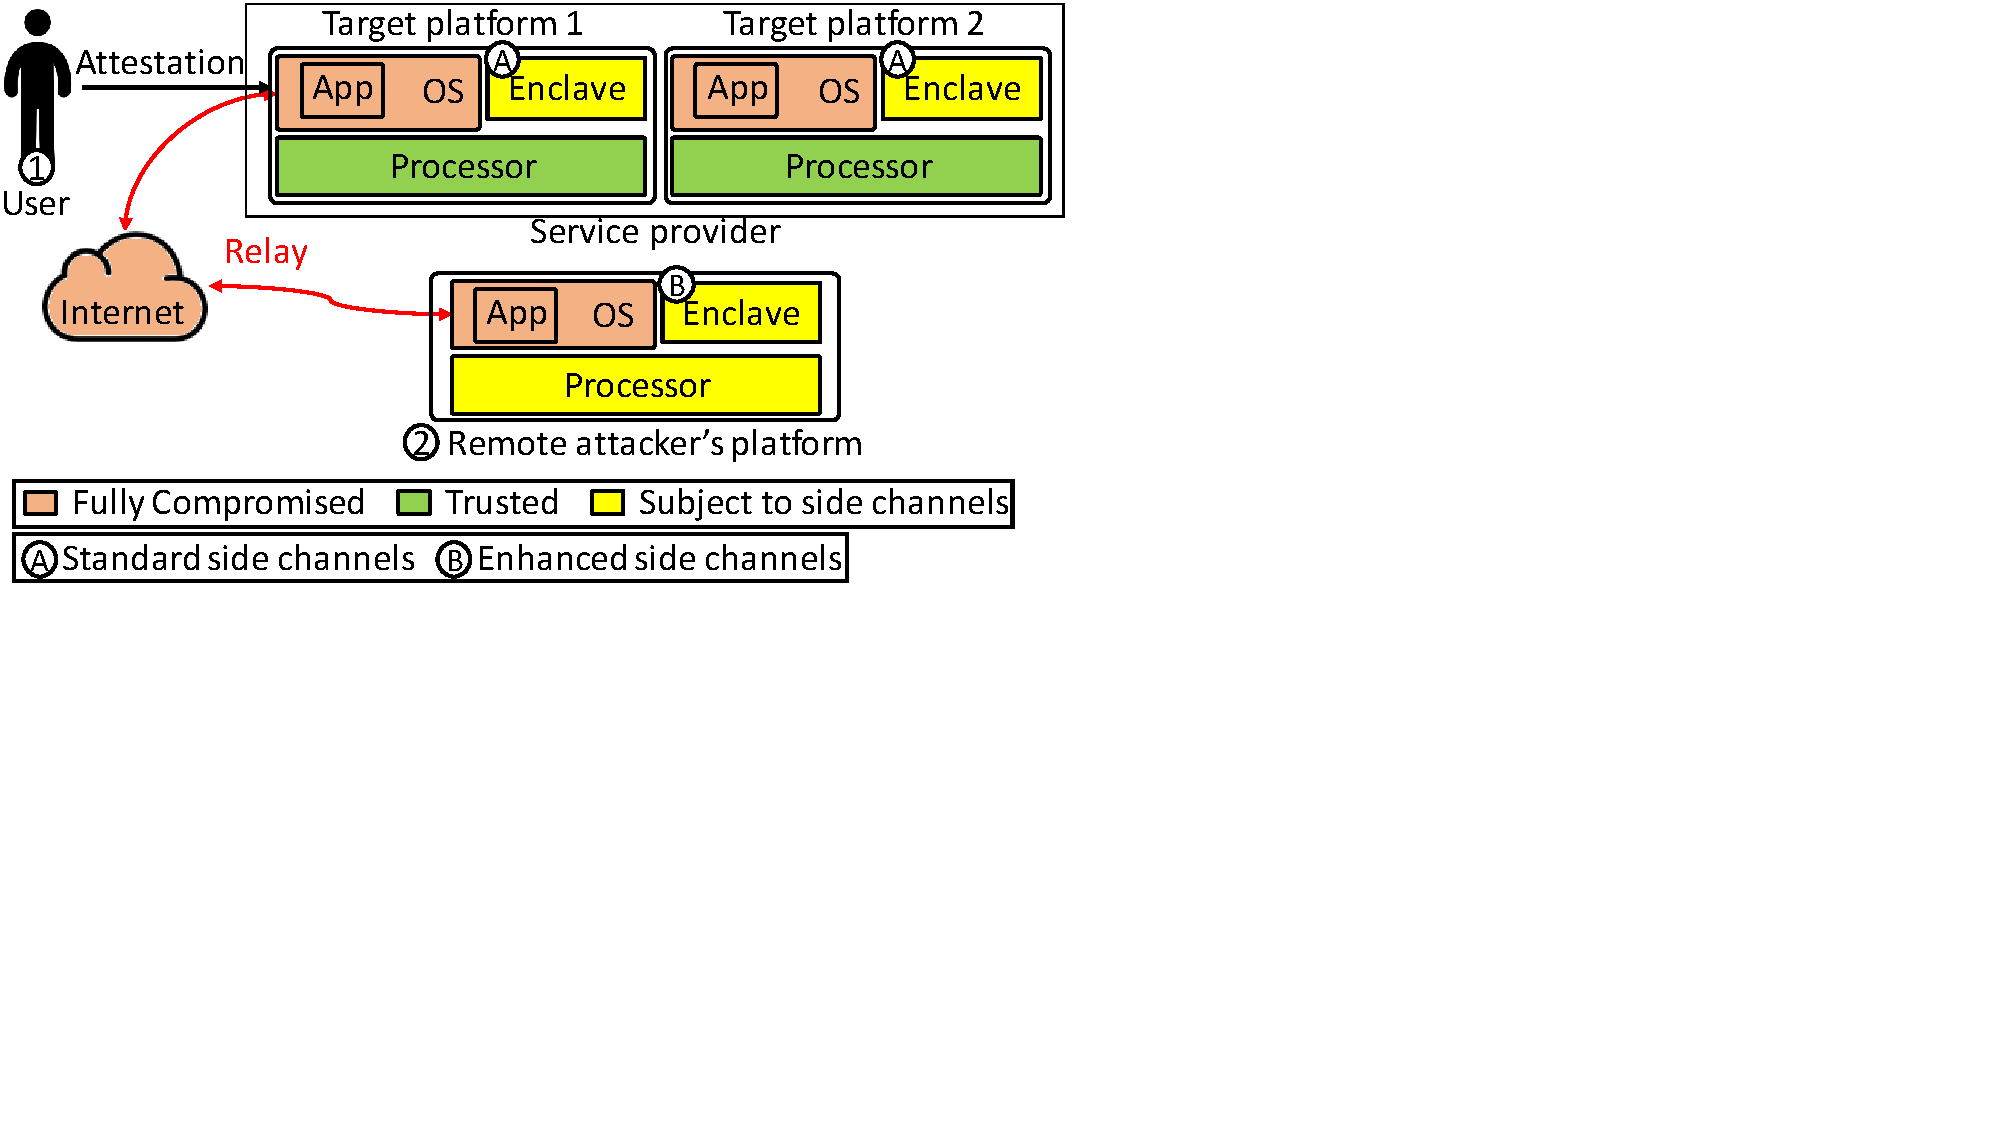
\includegraphics[trim={0cm 9cm 15.8cm 0},clip,width=0.9\linewidth]{relayAttack2.pdf}
 \caption{\textbf{Relay attack.} The adversary redirects attestation to his own platform which gives him increased (side-channel and kernel-level) abilities to attack the attested enclave.}
 \label{fig:SystemModel}
\end{figure}

\subsubsection*{Relay Attacks}

As shown in Figure~\ref{fig:SystemModel}... The relay attacker controls the OS and all other privileged software on the \emph{target} platform at least \emph{temporarily}, in particular at the time of the remote attestation. The OS compromise on the target platform may be later detected and disinfected. We consider the case in which the target platform resides in a data center or otherwise in a facility with restricted physical access. The attacker hence \emph{does not} have physical access to the target platform (or any other co-located platform in the same facility).
The relay attacker controls the OS and all other privileged software on the attacker's platform \emph{permanently} and has physical access to that platform. 

The relay attacker can redirect the attestation requests intended for the target platform to his platform, as shown in Figure~\ref{fig:SystemModel}. This is a realistic attack for two reasons. First, in the SGX attacker's model the adversary is allowed to control the OS and can hence easily redirect any network request the target platform receives. Second, even if the attacker cannot compromise the OS in the target platform, it might be able to exploit some vulnerability of the untrusted application managing the enclave. The exploit might allow the attacker to manipulate the application's control flow to redirect attestation request to any platform he desires.


\begin{figure}[t]
\footnotesize
    \centering
    \begin{tikzpicture}[
solved/.style={rectangle,draw,fill=purple!40, rounded corners, align=center},
not/.style={rectangle, draw,fill=orange!60, rounded corners, align=center},
neutral/.style={rectangle, draw, rounded corners, align=center, fill=black!5},
sibling distance=12em]]
    \node[neutral](root) {SGX attacks}
    child { node[not, yshift=13pt] (name) {Attacks enabled by \\ leaked attestation keys ~\cite{foreshadow-usenix18}} }
    child { node[neutral, yshift=13pt] (app) {Side-Channels \\ on application enclave}
      child { node[neutral, yshift=12pt] (soft) {Software/digital}
		child { node[solved, yshift=-4pt] (pe) {Privilege\\ escalation}}      
        child { node[not, right=1.5em of pe] (a) {Case (A):\\Complement of Case (B)}}
        child { node[solved, right=1.5em of a, yshift=-10pt] {Case (B):\\
            \begin{tabular}{rl}
                Target platform:& secure\\
                Attacker's platform:& vulnerable\\
            \end{tabular}}} }
      child { node[solved, yshift=12pt] (physical) {Physical} } };
      
    %\node[below=0cm of name] {Foreshadow~\cite{foreshadow-usenix18}};
    \node[below=0cm of physical](power) {Power analysis~\cite{wang2006covert}};
    \node[below=-5pt of power](EM) {EM radiation~\cite{gandolfi2001electromagnetic}};
    \node[below=-5pt of EM](ac) {Acoustic~\cite{shamir2004acoustic}};
         
    \node[left=10pt of soft](page) {Page fault~\cite{xu2015controlled}};
    \node[above=-3pt of page](cache) {Cache~\cite{dall2018cachequote}};
    \node[below=-2pt of page](branch) {Branch prediction~\cite{lee2017inferring}};
    %\node[below=-5pt of branch](synch) {Synchronization~\cite{asyncshock}};
      
    \node[solved, right=4em of root,  minimum size=3mm](l1) {};
    \node[right=0cm of l1](l1_1) {Enabled by relay};
    \node[not, below=1pt of l1, minimum size=3mm](l2) {};
    \node[right=0cm of l2](l2_1) {Independent of relay};
    
    \end{tikzpicture}
    
    \caption{\textbf{Relay attack implications.} The tree shows the types of attacks that are enabled by  redirection and ones that are independent of relay.}
    \label{fig:relayTree}
\end{figure}


\subsubsection*{Relay Attack Implications}            

Although relay attacks have been known for a long time~\cite{parno2008bootstrapping}, their implications to modern TEEs like SGX have not been carefully analyzed. Next, we perform the first such analysis.

The main consequence of attestation redirection is that it \emph{increases the adversary's ability to attack the attested enclave} through side-channels which are a well-known limitation of SGX. In Figure~\ref{fig:relayTree} we highlight two major classes of attacks: those that are only possible by first performing a relay attack, which we denote as ``enabled by relay'', and those that can be done whether or not the attacker also does a relay attack, which we call ``independent of relay.''

\paragraph{Attacks using leaked attestation keys.}
Our first observation is that attacks based on leaked attestation keys (e.g., ones obtained through the Foreshadow attack~\cite{foreshadow-usenix18}) are independent of relaying. If the adversary has obtained a valid and non-revoked attestation key, he can emulate an SGX processor on the target platform and obtain any secrets provisioned to it. %We revisit such emulation attacks and propose a solution for addressing them in Appendix~\ref{sec:variantII}. 

\paragraph{Physical side channels.}
One major benefit of the relay, from the adversary's point of view, is that it enables \emph{physical} side-channel attacks against application enclaves. Once a secret has been provisioned to the attacker's platform, she has as much time as she likes to perform the attack. Some examples of physical side-channel attacks are acoustic, electric and electromagnetic monitoring, which have been shown to be both effective and inexpensive means to extract secrets from modern PC platforms . Since the adversary does not have physical access to the target platform, such attacks are clearly not possible without relay. Hardening programs like enclaves against physical side channels is difficult and currently an open problem. Therefore, developers cannot easily defend their enclaves against physical side channels that are enabled by attestation redirection.

\paragraph{Privilege escalation for digital side channels.}
Another possible benefit of relay attacks is that it may enable \emph{privilege escalation}. In cases where the adversary has only compromised the user-space application that manages the enclave, and not the OS, the application can redirect the attestation to the attacker's remote platform where he controls the OS as well. In such cases, the relay enables \emph{digital} side-channel attacks that require system privileges.


\paragraph{Attacks that depend on timing of events.}    
The third, and perhaps the most subtle, implication of relay is that it can also enable software-based side-channel attacks that would not be possible to launch on the target platform due to \emph{timing of certain events}. These events include, but are not restricted to the provisioning of secrets to the enclave, the possible disinfection of the target platform from malicious software, and the discovery of a new side-channel attack. 

Case B is reached whenever it occurs that by using a side channel the enclave is exploitable on the attacker's platform, but not on the target platform. 
    A timeline of such case is shown in ..., where at the time of attestation and secret provisioning, the enclave is hardened against all known digital side-channel attacks (using tools like Raccoon~\cite{raccoon}). After secret provisioning, the OS compromise is detected and cleaned. Later, a new side-channel attack vector (that is not prevented by the used tools) is discovered. If the adversary performed redirection and the secret was provisioned to the attacker's machine, the new side channel is exploitable. Without the relay, the attack is not possible.



\subsubsection*{\namepm Design}

Our goal is to design a solution that addresses the limitations of the remote attestation Intel SGX i.e., vulnarable to the relay attack. In short, our solution should be \emph{secure} (no Trust on Fist Use (ToFU) assumption, small TCB, no online authorities) and \emph{easy to deploy} (no OS re-installation, manual configuration or pre-defined enclaves). In this section, we provide an overview of our proposed system: \namepm.

We propose a hardened SGX attestation scheme, called \namepm, based on a simple embedded device that we call \device. The embedded device is attached to the target platform over a local communication interface such as USB. 
Our main idea is to use the combination of such trusted device and \emph{proximity verification} to prevent relay attacks. In our solution, the \devicepm device verifies the proximity of the attested enclave and after successful proximity verification it facilitates the creation of a secure channel between the remote verifier and the attested enclave. 

After the initial attestation, the device periodically checks proximity to the attested enclave. The established secure channel is contingent on the physical presence of the embedded device on the target machine and it stays active only as long as the device is plugged-in. The act of detaching the device automatically revokes the attested platform without any interaction with a trusted authority. Thus, our solution enables secure \emph{offline} enrollment and revocation. 


\paragraph{Attestation Protocol} Figure~\ref{fig:systemSetUp} illustrates the \namepm attestation protocol that proceeds as follows:


\begin{figure}[t]
 \centering
  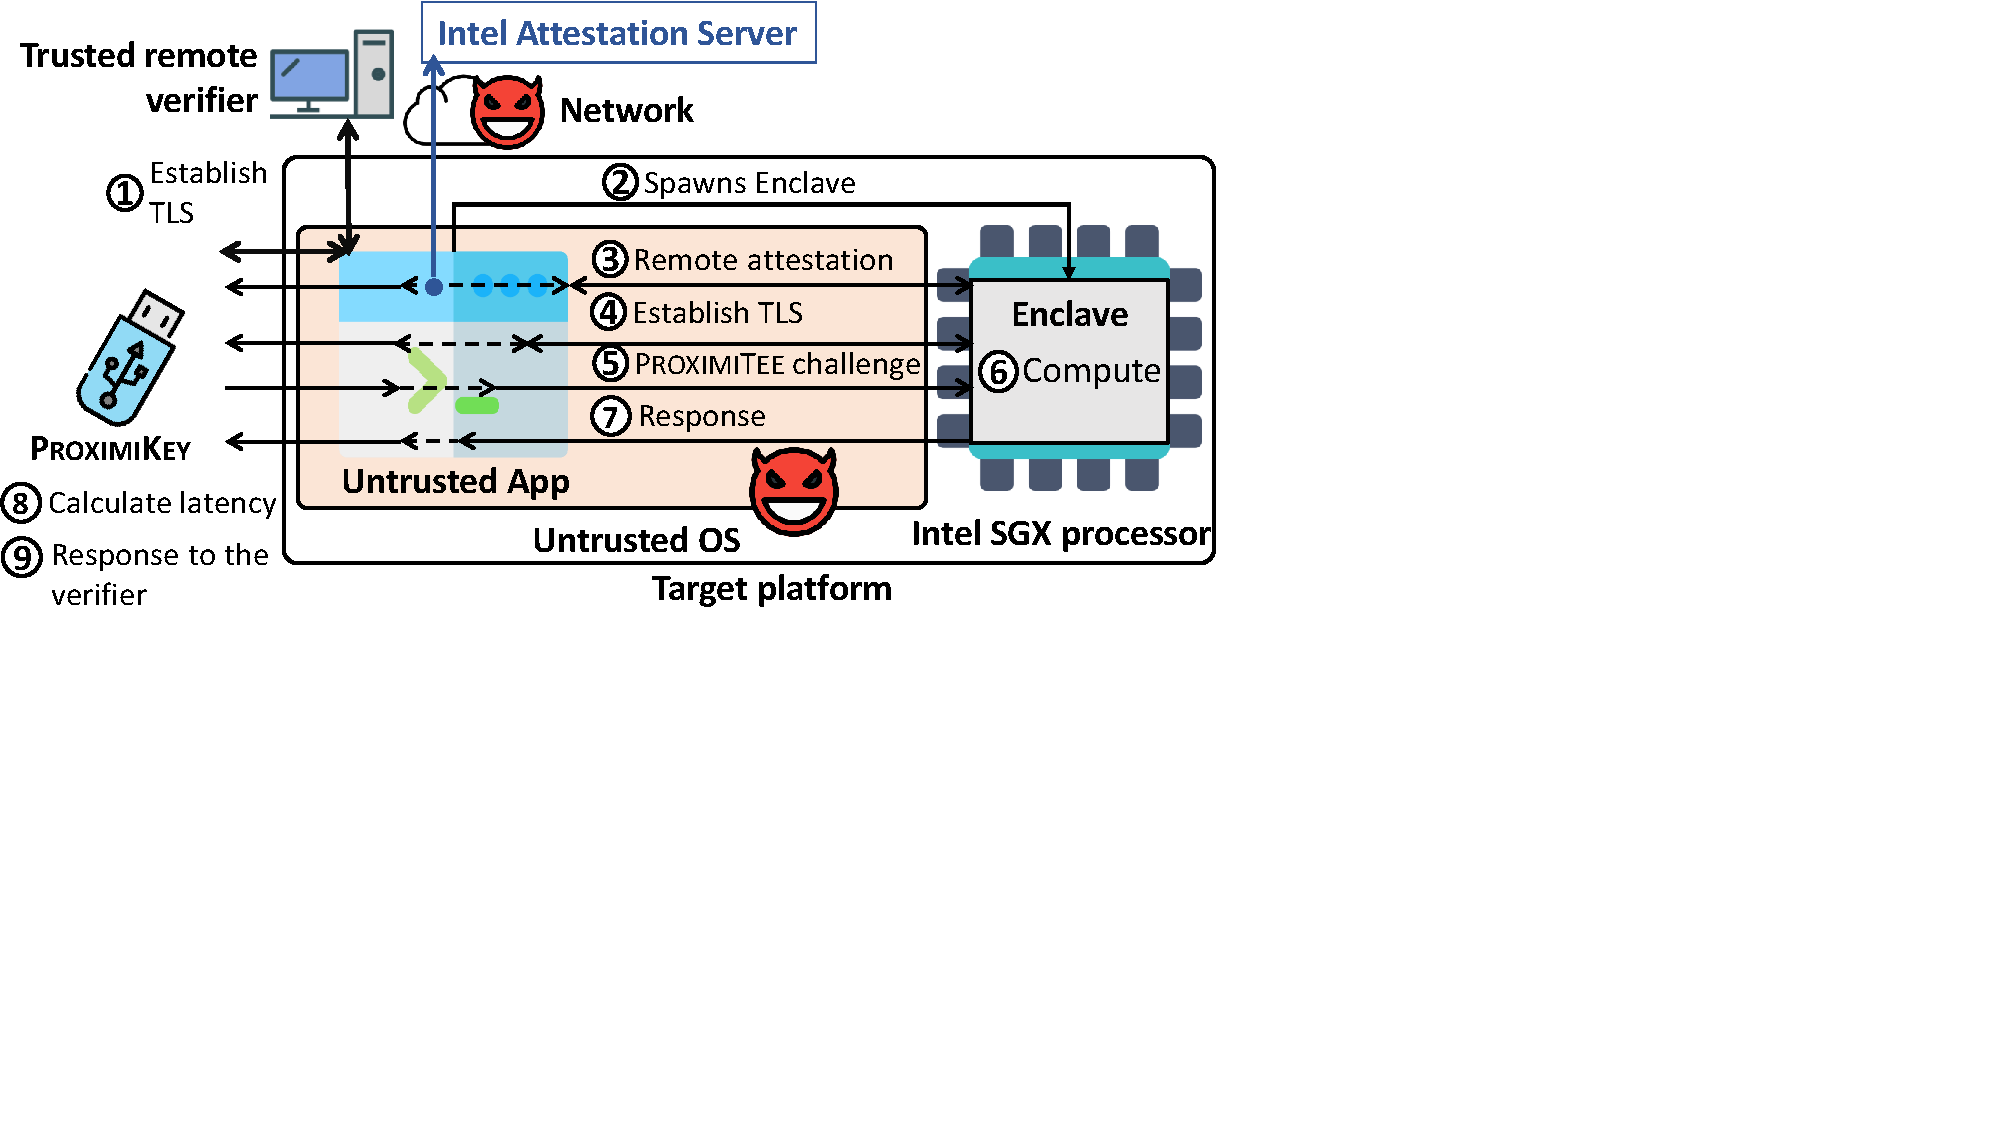
\includegraphics[trim={0 8.7cm 13.2cm 0},clip,width=\linewidth]{proximiteeMain.pdf}
 \caption{\textbf{\namepm attestation.} The remote verifier establishes a secure channel to the \devicepm device that first attests the enclave and then verifies its proximity.}
 \label{fig:systemSetUp}
\end{figure}

\begin{enumerate}
  \item[\one] The remote verifier establishes a secure channel (e.g., TLS) to the certified \devicepm. An assisting but untrusted user-space application facilitates the connection on the target platform acting as a transport channel between the remote verifier and the \devicepm (and later also the enclave). As part of this first step, the remote verifier specifies which enclave should be executed.

  \item[\two] The untrusted application creates and starts the attestation target enclave.

  \item[\three] \devicepm performs the standard remote attestation to verify the code configuration of the enclave with the help of the Intel Attestation Service (IAS) Server. In the attestation protocol, the device learns the public key of the attested enclave.

  \item[\four] \devicepm establishes a secure channel (e.g., TLS) to the enclave using that public key.

  \item[\five] \devicepm performs a distance-bounding protocol that consists of $n$ rounds, where each round is formed by steps \five to \eight.
  %(see Figure~\ref{fig:challengeResponse}).
  At the beginning of each round \devicepm generates a random challenge $r$ and sends it to the enclave over the TLS channel.

  \item[\six] The enclave increments the received challenge by one $(r+1)$.

  \item[\seven] The enclave sends a response ($r+1$) back to the \devicepm over the TLS channel.

  \item[\eight] \devicepm verifies that the response value is as expected (i.e., $r+1$) and checks if the latency of the response is below a threshold (\connect). Successful proximity verification requires that the latency is below the threshold for at least $k \times n$ responses, where $k \in (0, 1]$ is a percentage of the total number of responses $n$.

  \item[\nine] If proximity verification is successful, the \devicepm notifies the remote verifier over the TLS channel (constructed in step \one). The verifier starts using the \devicepm TLS channel to send messages to the enclave.
\end{enumerate}


\begin{figure}[t]
  \centering
    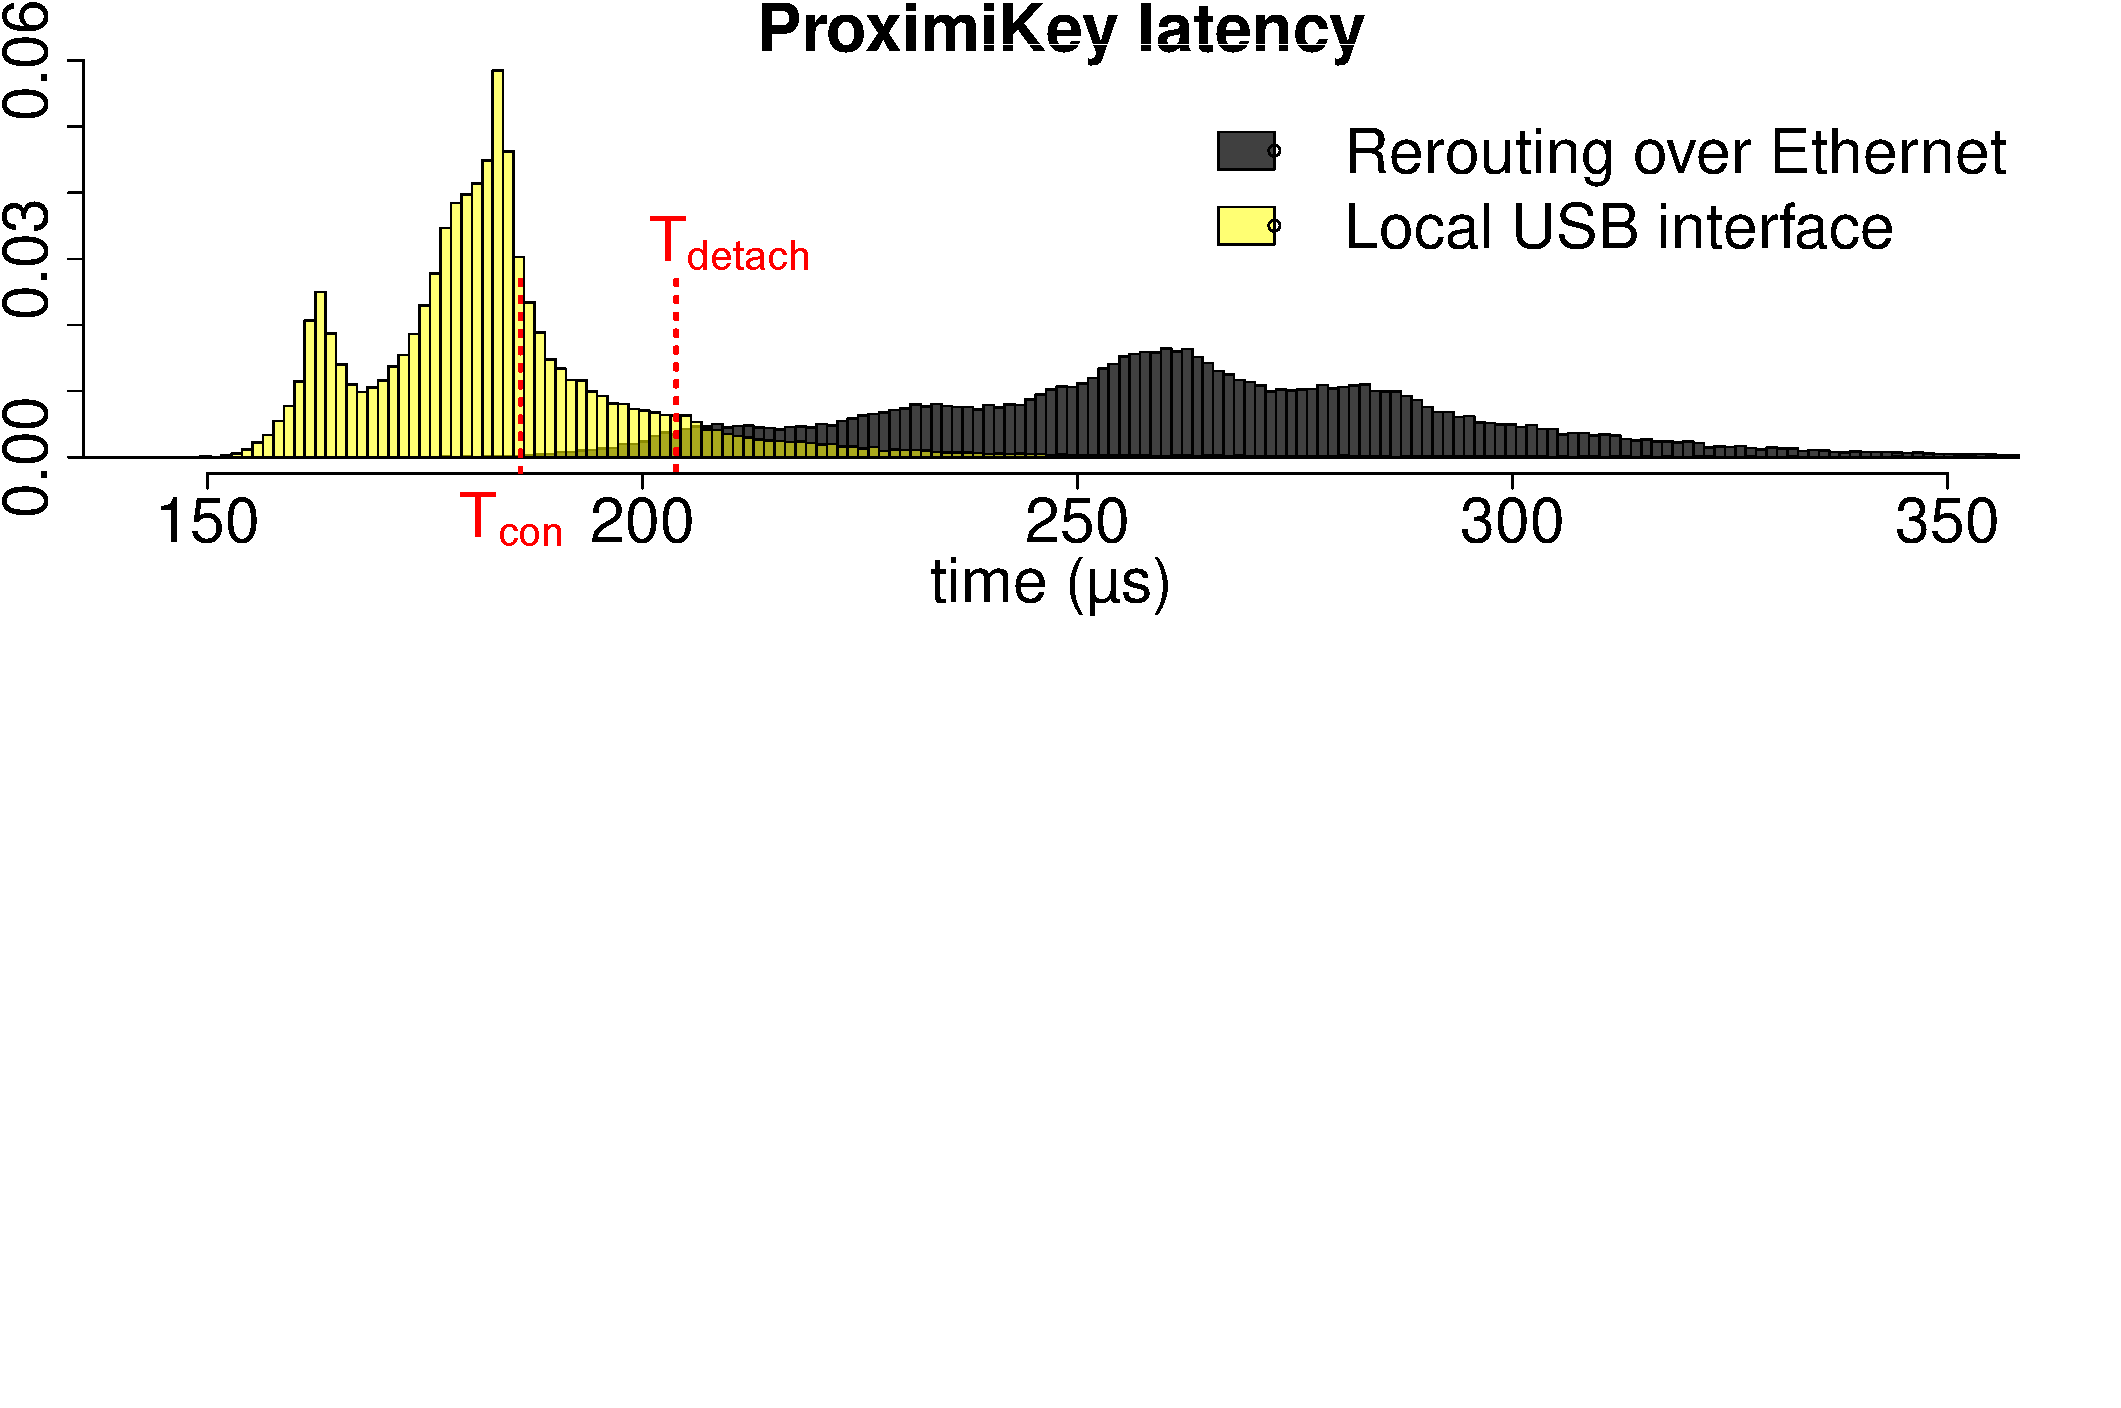
\includegraphics[trim={0 13.4cm 0 0},
    clip,width=\linewidth]{histo.pdf} 
    \caption{Latency distributions for legitimate challenge-response rounds and simulated relay attack.}
    \label{graph:instatAttackerHisto}
\end{figure}


\subsubsection*{Implementation}

We conducted our experiments on three SGX platforms...

The histogram in Figure~\ref{graph:instatAttackerHisto} on the left represents the challenge-response latencies in the legitimate proximity verification. The histogram on the right shows latencies in a simulated attack (including a post-processing phase where we reduce the adversary's measured network latencies to half to accommodate the assumption of the attacker's infinitely fast network interface).

As can be seen from Figure~\ref{graph:instatAttackerHisto}, the vast majority of the benign challenge-responses take from $145$ to $250 \mu s$. The vast majority of the round-trip times in the simulated attack take from $200$ to $750$ $\mu s$. Hence, the average delay of our simulated adversary is only $80 \mu s$. To put this into perspective, even the highly-optimized network connections between major data centers in the same region exhibit latencies from one millisecond upwards which is one order of magnitude more than in our simulated setup.

\paragraph{Results} We simulate a powerful relay-attack adversary that is connected to the target platform with fast network connection. To consider the best case for the adversary, we make several assumptions in his favor. For example, we assume that he can instantly perform all computations needed to participate in the proximity verification protocol. However, he cannot break cryptographic hardness assumptions. We define the adversary's success as the event in which proximity verification succeeds with an enclave that resides on the attacker's platform and denote the probability of such event $P_{adv}$. We define the legitimate success as the event in which proximity verification succeeds with an enclave that resides in the target platform and denote its probability $P_{legit}$. We saw that it is possible to find parameters ($n=50$, $k=0.3$ and \connect$=186 \mu s$) that make proximity verification very secure ($P_{adv}=3.55\times 10^{-34}$) and reliable ($P_{legit}=0.999999977$).




